\documentclass[DaoFP]{subfiles}
\begin{document}
\setcounter{chapter}{1}
\chapter{Composition}

\section{Composition}

Programming is about composition. Paraphrasing Wittgenstein, one could say: ``Of that which cannot be decomposed one should not speak.'' This is not a prohibition, it's a statement of fact. The process of studying, understanding, and describing is the same as the process of decomposing; and our language reflects this. 

The reason we have built the vocabulary of objects and arrows is precisely to express the idea of composition.  

Given an arrow $f$ from $a$ to $b$ and an arrow $g$ from $b$ to $c$, their composition is an arrow that goes directly from $a$ to $c$. In other words, if there are two arrows, the target of one being the same as the source of the other, we can always compose them to get a third arrow.

\[
 \begin{tikzcd}
 a
 \arrow[rr, bend left, "h"]
 \arrow[r, "f"']
 & b
 \arrow[r, "g"']
& c
 \end{tikzcd}
\]

In math we denote composition using a little circle
\[h = g \circ f\]
We read this: ``$h$ is equal to $g$ after $f$.'' The choice of the word ``after'' suggests temporal ordering of actions, which in most cases is a useful intuition.

The order of composition might seem backward, but this is because we think of functions as taking arguments on the right.
In Haskell we replace the circle with a dot:
\begin{haskell}
h = g . f
\end{haskell}
This is every program in a nutshell. In order to accomplish \hask{h}, we decompose it into simpler problems, \hask{f} and \hask{g}. These, in turn, can be decomposed further, and so on.

Now suppose that we were able to decompose $g$ itself into $j \circ k$. We have
\[h = (j \circ k) \circ f\]
We want this decomposition to be the same as
\[h = j \circ (k \circ f)\]
We want to be able to say that we have decomposed $h$ into three simpler problems
\[h =  j \circ k \circ f\]
and not have to keep track which decomposition came first. This is called \emph{associativity} of composition, and we will assume it from now on.

Composition is the source of two mappings of arrows called pre-composition and post-composition. 

When you \index{post-composition}\emph{post-compose} an arrow $h$ with an arrow $f$, it produces the arrow $f \circ h$ (the arrow $f$ is applied \emph{after} the arrow $h$). Of course, you can post-compose $h$ only with arrows whose source is the target of $h$. Post-composition by $f$ is written as $(f \circ -)$, leaving a hole for $h$. As Lao Tzu would say, ``Usefulness of post-composition comes from what is not there.''

Thus an arrow $f \colon a \to b$ induces a mapping of arrows $(f \circ -)$ that maps arrows which are probing $a$ to arrows which are probing $b$. 

\[
 \begin{tikzcd}
 \node (a1) at (0, 2) {};
 \node (a2) at (-0.5, 2) {};
 \node (a3) at (0.5, 2) {};
 \node (aa) at (0.5, 1) {};
 \node(a) at (0, 0) {a};
 \draw[->, red] (a1) -- (a);
 \draw[->] (a2) -- (a);
 \draw[->, blue] (a3) -- (a);
 \node (b1) at (3+0, 2) {};
 \node (b2) at (3-0.5, 2) {};
 \node (b3) at (3+0.5, 2) {};
 \node (bb) at (2.5, 1) {};
 \node(b) at (3, 0) {b};
 \draw[->, red] (b1) -- (b);
 \draw[->] (b2) -- (b);
 \draw[->, blue] (b3) -- (b);
 \draw[->] (a) -- node[below]{f} (b);
 \draw[->, dashed] (aa) -- node[above]{(f \circ -)} (bb);
  \end{tikzcd}
\]
Since objects have no \emph{internal} structure, when we say that $f$ transforms $a$ to $b$, this is exactly what we mean. 

Post-composition lets us shift focus from one object to another.

Dually, you can \index{pre-composition}\emph{pre-compose} by $f$, or apply $(- \circ f)$ to arrows originating in $b$ to map them to arrows originating in $a$ (notice the change of direction). 

\[
 \begin{tikzcd}
 \node (a1) at (0, -2) {};
 \node (a2) at (-0.5, -2) {};
 \node (a3) at (0.5, -2) {};
 \node (aa) at (0.5, -1) {};
 \node(a) at (0, 0) {a};
 \draw[<-, red] (a1) -- (a);
 \draw[<-] (a2) -- (a);
 \draw[<-, blue] (a3) -- (a);
 \node (b1) at (3+0, -2) {};
 \node (b2) at (3-0.5, -2) {};
 \node (b3) at (3+0.5, -2) {};
 \node (bb) at (2.5, -1) {};
 \node(b) at (3, 0) {b};
 \draw[<-, red] (b1) -- (b);
 \draw[<-] (b2) -- (b);
 \draw[<-, blue] (b3) -- (b);
 \draw[->] (a) -- node[above]{f} (b);
 \draw[->, dashed] (bb) -- node[below]{(- \circ f)} (aa);
  \end{tikzcd}
\]

Pre-composition lets us shift the perspective from observer $b$ to observer $a$.

Pre- and post-composition are mappings of arrows. Since arrows form sets, these are \emph{functions} between sets. 

Another way of looking at pre- and post-composition is that they are the result of partial application of the two-hole composition operator $(- \circ -)$, in which we can pre-fill one hole or the other with a fixed arrow.

In programming, an outgoing arrow is interpreted as extracting data from its source. An incoming arrow is interpreted as producing or constructing the target. Outgoing arrows define the interface, incoming arrows define the constructors.

For Haskell programmers, here's the implementation of post-composition as a higher-order function:
\begin{haskell}
postCompWith :: (a -> b) -> (x -> a) -> (x -> b)
postCompWith f = \h -> f . h
\end{haskell}
And similarly for pre-composition:
\begin{haskell}
preCompWith :: (a -> b) -> (b -> x) -> (a -> x)
preCompWith f = \h -> h . f
\end{haskell}

Do the following exercises to convince yourself that shifts in focus and perspective are composable.
\begin{exercise}\label{ex-yoneda-composition}
Suppose that you have two arrows, $f \colon a \to b$ and $g \colon b \to c$. Their composition $g \circ f$ induces a mapping of arrows $((g \circ f) \circ -)$. Show that the result is the same if you first apply $(f \circ -)$ and follow it by $(g \circ -)$. Symbolically:
\[((g \circ f) \circ -) = (g \circ -) \circ (f \circ -)\]

Hint: Pick an arbitrary object $x$ and an arrow $h \colon x \to a$ and see if you get the same result. Note that $\circ$ is overloaded here. On the right, it means regular function composition when put between two post-compositions.
\end{exercise}

\begin{exercise}
Convince yourself that the composition from the previous exercise is associative. Hint: Start with three composable arrows.
\end{exercise}

\begin{exercise}
Show that pre-composition $(- \circ f)$ is composable, but the order of composition is reversed:
\[(- \circ (g \circ f)) = (- \circ f) \circ (- \circ g) \]
\end{exercise}

\section{Function application}

We are ready to write our first program. There is a saying: ``A journey of a thousand miles begins with a single step.'' Consider a journey from $1$ to $b$. Our single step can be an arrow from the terminal object $1$ to some $a$. It's an element of $a$. We can write it as:
\[1 \xrightarrow x a \]
The rest of the journey is the arrow:
\[a \xrightarrow f b\]
These two arrows are composable (they share the object $a$ in the middle) and their composition is the arrow $y$ from $1$ to $b$. In other words, $y$ is an \emph{element} of $b$:

\[
 \begin{tikzcd}
 1
 \arrow[rr, bend left, "y"]
 \arrow[r, "x"']
 & a
 \arrow[r, "f"']
& b
 \end{tikzcd}
\]
We can write it as:
\[y = f \circ x \]

We used $f$ to map an \emph{element} of $a$ to an \emph{element} of $b$. Since this is something we do quite often, we call it the \emph{application} of a function $f$ to $x$, and use the shorthand notation
\[y = f x \]
Let's translate it to Haskell. We start with an element $x$ of $a$ (a shorthand for \hask{x :: ()-> a})
\begin{haskell}
x :: a
\end{haskell}
We declare a function $f$ as an element of the ``object of arrows'' from $a$ to $b$
\begin{haskell}
f :: a -> b
\end{haskell}
with the understanding (which will be elaborated upon later) that it corresponds to an arrow from \hask{a} to \hask{b}. The result is an element of $b$
\begin{haskell}
y :: b
\end{haskell}
and it is defined as
\begin{haskell}
y = f x
\end{haskell}
We call this the application of a function to an argument, but we were able to express it purely in terms of function composition. (Note: In other programming languages function application requires the use of parentheses, e.g., \hask{y = f(x)}.)

\section{Identity}

You may think of arrows as representing change: object $a$ becomes object $b$. An arrow that loops back represents a change in an object itself. But change has its dual: lack of change, inaction or, as Lao Tzu would say \emph{wu wei}. 

Every object has a special arrow called the identity, which leaves the object unchanged. It means that, when you compose this arrow with any other arrow, either incoming or outgoing, you get that other arrow back. Thought of as an action, the identity arrow does nothing and takes no time.

An identity arrow on the object $a$ is called $id_a$. So if we have an arrow $f \colon a \to b$, we can compose it with identities on either side

\[id_b \circ f = f = f \circ id_a \]
or, pictorially:
\[
 \begin{tikzcd}
 a
 \arrow[loop, "id_a"']
 \arrow[r, "f"]
 & b
 \arrow[loop, "id_b"']
 \end{tikzcd}
\]

We can easily check what an identity does to elements. Let's take an element $x \colon 1 \to a$ and compose it with $id_a$. The result is:
\[id_a \circ x = x\]
which means that identity leaves elements unchanged.

In Haskell, we use the same name \hask{id} for all identity functions (we don't subscript it with the type it's acting on). The above equation, which specifies the action of $id$ on elements, translates directly to:
\begin{haskell}
id x = x
\end{haskell}
and it becomes the definition of the function \hask{id}. 

We've seen before that both the initial object and the terminal object have unique arrows circling back to them. Now we are saying that every object has an identity arrow circling back to it. Remember what we said about uniqueness: If you can find two of those, then they must be equal. We must conclude that these unique looping arrows we talked about must be the identity arrows. We can now label these diagrams:

\[
 \begin{tikzcd}
 \hask{Void}
 \arrow[loop, "id"']
 \end{tikzcd}
 \begin{tikzcd}
 \hask{()}
 \arrow[loop, "id"']
 \end{tikzcd}
\]

In logic, identity arrow translates to a tautology. It's a trivial proof that, ``if $a$ is true then $a$ is true.'' It's also called the \emph{identity rule}.


If identity does nothing then why do we care about it? Imagine going on a trip, composing a few arrows, and finding yourself back at the starting point. The question is: Have you done anything, or have you wasted your time? The only way to answer this question is to compare your path to the identity arrow. 

Some round trips bring change, others don't.

More importantly, identity arrows will allow us to compare objects. They are an integral part of the definition of an isomorphism.

\begin{exercise}\label{ex-yoneda-identity}
What does $(id_a \circ -)$ do to arrows terminating in $a$? What does $(- \circ id_a)$ do to arrows originating from $a$?
\end{exercise}

\section{Monomorphisms}

Consider the function \hask{even} that tests whether its input is divisible by two:
\begin{haskell}
even :: Int -> Bool
\end{haskell}
It's a many-to-one function: all even numbers are mapped to \hask{True} and all odd numbers to \hask{False}. Most information about the input is discarded, we are only interested in its evenness, not its actual value. By discarding information we arrive at an abstraction\footnote{to abstract literally means to draw away}. Functions (and later functors) epitomize abstractions.

Contrast this with the function \hask{injectBool}:
\begin{haskell}
injectBool :: Bool -> Int
injectBool b = if b then 1 else 0
\end{haskell}
This function doesn't discard information. You can recover its argument from its result. 

Functions that don't discard information are also useful: they can be thought of as injecting their source into their target. You may imagine the type of the source as a \emph{shape} that is being embedded in the target. Here, we are embedding a two-element shape \hask{Bool} into the type of integers. 

\[
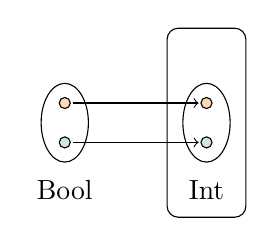
\begin{tikzpicture}
   \def\Xa{0};
   \def\Xb{1.8}       
   \def\Y{0};
   \def\Yb{-0.85};
   \def\delta{0.1};
  
         \draw(\Xa, \Y) ellipse (0.3 and 0.5);
	% dots
        \draw (\Xa, \Y + 0.25) [fill=orange!30] circle (2pt);
        \draw (\Xa, \Y - 0.25) [fill=blue!50!green!20] circle (2pt);
        
        \draw [rounded corners] (\Xb - 0.5, \Y - 1.2) rectangle (\Xb + 0.5, \Y + 1.2) {};
        \draw(\Xb, \Y) ellipse (0.3 and 0.5);
	% dots
        \draw (\Xb, \Y + 0.25) [fill=orange!30] circle (2pt);
        \draw (\Xb, \Y - 0.25) [fill=blue!50!green!20] circle (2pt);
        % arrows
        \draw [->] (\Xa + \delta, \Y - 0.25) -- (\Xb - \delta, \Y - 0.25);
        \draw [->] (\Xa + \delta, \Y + 0.25) -- (\Xb - \delta, \Y + 0.25);
        % labels
        \node at (\Xa, \Yb) {Bool};
        \node at (\Xb, \Yb) {Int};
\end{tikzpicture}
\]

Injective functions, or \index{injections}\emph{injections} are defined to always assign different values to different arguments. In other words, they don't collapse multiple elements into one. 

Here's another, slightly convoluted, way of saying this: An injection maps two elements to one only when the two elements are equal. 

We could translate this definition to the categorical language by replacing ``elements'' with arrows from the terminal object. We would say that $f \colon a \to b$ is an injection if, for any pair of global elements $x_1 \colon 1 \to a$ and $x_2 \colon 1 \to a$, the following implication holds:
\[ f \circ x_1 = f \circ x_2 \implies x_1 = x_2 \]

\[
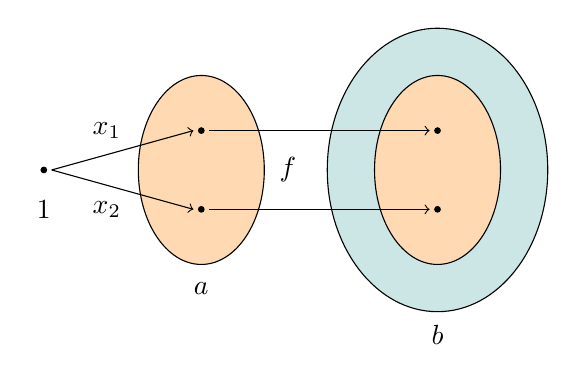
\begin{tikzpicture}
  \def\X{-2.0}
  \def\Xa{0};
  \def\Xmid{1.1};
  \def\Xb{3};
  \def\delta{0.1};
  
  \def\Ymid{0};
  \def\Ytip{-0.9};
  \def\Ybot{-1.5};
         \draw (\Xa , \Ymid)[fill=orange!30]  ellipse (0.8 and 1.2);
         \draw (\Xb, \Ymid)[fill=blue!50!green!20]   ellipse (1.4 and 1.8);
         \draw (\Xb , \Ymid) [fill=orange!30]  ellipse (0.8 and 1.2);
	% dots
        \filldraw (\X, \Ymid) circle (1pt);
        \filldraw (\Xa, \Ymid - 0.5) circle (1pt);
        \filldraw (\Xa, \Ymid + 0.5) circle (1pt);
        \filldraw (\Xb, \Ymid - 0.5) circle (1pt);
        \filldraw (\Xb, \Ymid + 0.5) circle (1pt);

	% arrows 
	\draw [->] (\X + \delta, \Ymid) --  (\Xa - \delta, \Ymid + 0.5);
	\draw [->] (\X + \delta, \Ymid)  -- (\Xa - \delta, \Ymid - 0.5);
	\draw [->] (\Xa + \delta, \Ymid + 0.5) --  (\Xb - \delta, \Ymid + 0.5);
	\draw [->] (\Xa + \delta, \Ymid - 0.5)  -- (\Xb - \delta, \Ymid - 0.5);
	
	% labels
	\node at (\Xmid, \Ymid) { $f$ };
	\node at (\X + 0.8, \Ymid + 0.5) { $x_1$ };
	\node at (\X + 0.8, \Ymid - 0.5) { $x_2$ };
	\node at (\X, \Ymid - 0.5) {$1$};
	\node at (\Xa, \Ybot) {$a$};
	\node at (\Xb, \Ybot - 0.6) {$b$};

\end{tikzpicture}
\]

The problem with this definition is that not every category has a terminal object. A better definition would replace global elements with arbitrary shapes. Thus the notion of injectivity is generalized to that of monomorphism. 

An arrow $f \colon a \to b$ is  \index{monomorphism}\emph{monomorphic} if, for any choice of an object $c$ and a pair of arrows $g_1 \colon c \to a$ and $g_2 \colon c \to a$ we have the following implication:
\[ f \circ g_1 = f \circ g_2 \implies g_1 = g_2 \]

To show that an arrow $f \colon a \to b$ is \emph{not} a monomorphism, it's enough to find a counterexample: two different shapes in $a$, such that $f$ maps them to the same shape in $b$. 

Monomorphisms, or ``monos'' for short, are often denoted using special arrows, as in $a \hookrightarrow b$ or $a \rightarrowtail b$. 

In category theory objects are indivisible, so we can only talk about sub-objects using arrows. We say that monomorphism $a \hookrightarrow b$ picks a subobject of $b$ in the shape of $a$.

\begin{exercise}
Show that any arrow from the terminal object is a monomorphism.
\end{exercise}

\section{Epimorphisms}

The function \hask{injectBool} is injective (hence a monomorphism), but it only covers a small subset of its target --- just two integers out of infinitely many.
\begin{haskell}
injectBool :: Bool -> Int
injectBool b = if b then 1 else 0
\end{haskell}
In contrast, the function \hask{even} covers the whole of \hask{Bool} (it can produce both \hask{True} and \hask{False}). A function that covers the whole of its target is called a \index{surjection}\emph{surjection}.

To generalize injections we used additional mappings-in. To generalize surjections, we'll use mappings-out. The categorical counterpart of a surjection is called an epimorphism.

An arrow $f \colon a \to b$ is an \index{epimorphism}\emph{epimorphism} if for any choice of an object $c$ and a pair of arrows $g_1 \colon b \to c$ and $g_2 \colon b \to c$ we have the following implication:
\[ g_1 \circ f = g_2 \circ f \implies g_1 = g_2 \]
Conversely, to show that $f$ is not an epimorphism, it's enough to pick an object $c$ and two different arrows $g_1$ and $g_2$ that agree when precomposed with $f$.

To get some insight into this definition, we have to visualize mappings out. Just as a mapping into an object can be thought of as defining a shape, mapping out of an object can be thought of as defining properties of that object. 

This is clear when dealing with sets, especially if the target set is finite. You may think of an element of the target set as defining a color. All elements of the source that are mapped to that element are ``painted'' a particular color. For instance, the function \hask{even} paints all even integers the \hask{True} color, and all odd ones the \hask{False} color.

In the definition of an epimorphism we have two such mapping, $g_1$ and $g_2$. Suppose that they differ only slightly. Most of the object $b$ is painted alike by both of them.

\[
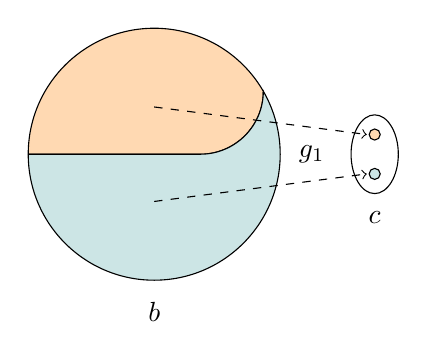
\begin{tikzpicture}
  \def\Xa{0};
  \def\Xmid{1.2};
  \def\Xb{3.2};
  \def\Xc{6};
  \def\delta{0.1};
  \def\d{0.3};
  \def\R{0.8};
  
  \def\Y{0};
  \def\Ybot{-2};
  
         \draw(\Xc, \Y) ellipse (0.3 and 0.5);
         % areas
        \draw [fill=orange!30] (\Xb - 2 * \R, \Y) 
        arc[start angle=180, delta angle=-180+30, radius=2 * \R]
        arc[start angle=0, delta angle=-90, radius=\R]
         to (\Xb - 2 * \R, \Y);
         
         \draw [fill=blue!50!green!20]  (\Xb - 2 * \R, \Y)
         arc[start angle=-180, delta angle=180+30, radius=2 * \R]
         arc[start angle=0, end angle=-90, radius=\R] 
         to (\Xb - 2 * \R, \Y);

	% dots
        \draw (\Xc, \Y + 0.25) [fill=orange!30] circle (2pt);
        \draw (\Xc, \Y - 0.25) [fill=blue!50!green!20] circle (2pt);

	% arrows
	\draw[->, dashed] (\Xb, \Y + 0.6) -- (\Xc - \delta, \Y + 0.25);
	\draw[->, dashed] (\Xb, \Y - 0.6) -- (\Xc - \delta, \Y - 0.25);
	% labels
	\node at (\Xc - 0.8, \Y) { $g_1$ };
	\node at (\Xb, \Ybot) {$b$};
	\node at (\Xc, \Y - 0.8) {$c$};
\end{tikzpicture}
\hspace{1cm}
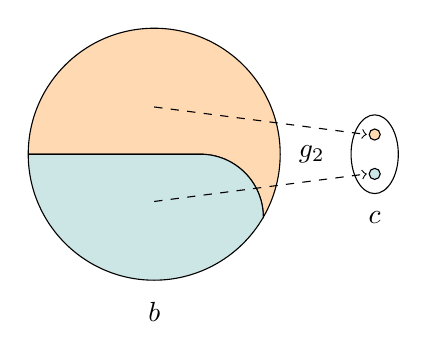
\begin{tikzpicture}

  \def\Xa{0};
  \def\Xmid{1.2};
  \def\Xb{3.2};
  \def\Xc{6};
  \def\delta{0.1};
  \def\d{0};
  \def\R{0.8};
  
  \def\Y{0};
  \def\Ybot{-2};
  
         \draw(\Xc, \Y) ellipse (0.3 and 0.5);
         % areas
          \draw [fill=orange!30] (\d + \Xb - 2 * \R, \Y) 
         arc[start angle=180, delta angle=-180-30, radius=2 * \R]
         arc[start angle=0, delta angle=90, radius=\R]
         to (\d + \Xb - 2 * \R, \Y);
         
         \draw [fill=blue!50!green!20]  (\d + \Xb - 2 * \R, \Y)
         arc[start angle=-180, delta angle=180-30, radius=2 * \R]
         arc[start angle=0, end angle=90, radius=\R] 
         to (\d + \Xb - 2 * \R, \Y);
         
	% dots
        \draw (\Xc, \Y + 0.25) [fill=orange!30] circle (2pt);
        \draw (\Xc, \Y - 0.25) [fill=blue!50!green!20] circle (2pt);
        
	% arrows
	\draw[->, dashed] (\Xb, \Y + 0.6) -- (\Xc - \delta, \Y + 0.25);
	\draw[->, dashed] (\Xb, \Y - 0.6) -- (\Xc - \delta, \Y - 0.25);
	% labels
	\node at (\Xc - 0.8, \Y) { $g_2$ };
	\node at (\Xb, \Ybot) {$b$};
	\node at (\Xc, \Y - 0.8) {$c$};
\end{tikzpicture}
\]

If $f$ is \emph{not} an epimorphism, it's possible that its image only covers the part that is painted alike by $g_1$ and $g_2$. The two arrows then agree on painting $a$ when precomposed by $f$, even though they are different on the whole.


\[
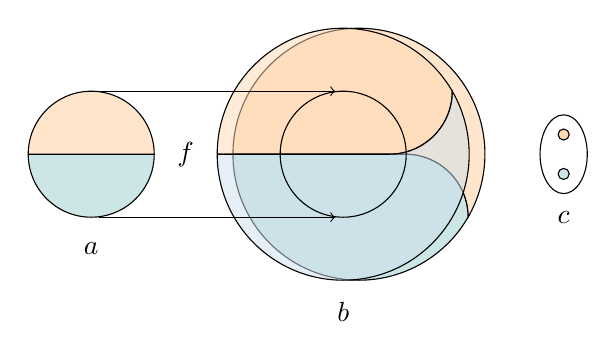
\begin{tikzpicture}
  \def\Xa{0};
  \def\Xmid{1.2};
  \def\Xb{3.2};
  \def\Xc{6};
  \def\delta{0.1};
  \def\d{0.2};
  \def\R{0.8};
  
  \def\Y{0};
  \def\Ymid{-1.2};
  \def\Ybot{-2};
  
         % \draw (\Xa , \Y)  circle ( \R);
         \draw [fill=blue!50!green!20] (\Xa - \R, \Y)
         arc[start angle = -180, delta angle = 180, radius = \R]
         to (\Xa - \R, \Y);
         \draw [fill=orange!20] (\Xa - \R, \Y)
         arc[start angle = -180, delta angle = -180, radius = \R]
         to (\Xa - \R, \Y);
         
         \draw(\Xc, \Y) ellipse (0.3 and 0.5);
         % area right
          \draw [fill=orange!20] (\d + \Xb - 2 * \R,  \Y) 
         arc[start angle=180, delta angle=-180-30, radius=2 * \R]
         arc[start angle=0, delta angle=90, radius=\R]
         to (\d + \Xb - 2 * \R, \Y);
         
         \draw [fill=blue!50!green!20]  (\d + \Xb - 2 * \R, \Y)
         arc[start angle=-180, delta angle=180-30, radius=2 * \R]
         arc[start angle=0, end angle=90, radius=\R] 
         to (\d + \Xb - 2 * \R, \Y);
	% area left
        \draw [fill=orange!30, fill opacity=0.5] (\Xb - 2 * \R, \Y) 
        arc[start angle=180, delta angle=-180+30, radius=2 * \R]
        arc[start angle=0, delta angle=-90, radius=\R]
         to (\Xb - 2 * \R, \Y);
         
         \draw [fill=blue!60!green!20, fill opacity=0.5]  (\Xb - 2 * \R, \Y)
         arc[start angle=-180, delta angle=180+30, radius=2 * \R]
         arc[start angle=0, end angle=-90, radius=\R] 
         to (\Xb - 2 * \R, \Y);

         \draw (\Xb , \Y)  circle ( \R);
         
	% dots
        \draw (\Xc, \Y + 0.25) [fill=orange!30] circle (2pt);
        \draw (\Xc, \Y - 0.25) [fill=blue!50!green!20] circle (2pt);
        
        %\filldraw (\Xb + \R + 0.7 * \R, \Y + 0.1)  circle (1pt);

	% arrows 
	\draw [->] (\Xa + \delta, \Y + \R) --  (\Xb - \delta, \Y + \R);
	\draw [->] (\Xa + \delta, \Y - \R)  -- (\Xb - \delta, \Y - \R);
	
	% labels
	\node at (\Xmid, \Y) { $f$ };
	\node at (\Xa, \Ymid) {$a$};
	\node at (\Xb, \Ybot) {$b$};
	\node at (\Xc, \Y - 0.8) {$c$};

\end{tikzpicture}
\]
Of course, this is just an illustration. In an actual category there is no peeking inside objects.

Epimorphisms, or ``epis'' for short, are often denoted by a special arrow $a \twoheadrightarrow b$.

In sets, a function that is both injective and surjective is called a bijection. It provides a one-to-one invertible mapping between elements of two sets. This role is played by isomorphisms in category theory. However, in general it's not true that an arrow that is both mono and epi is an isomorphism.

\begin{exercise}
Show that any arrow to the terminal object is an epimorphism.
\end{exercise}


\end{document}